\section{Mobility Datasets}

% Why do we need this dataset?
In order to get insights about the possible impact of changed mobility behavior on greenhouse gas emissions, it is important to use different kind of mobility data. The goal by using those datasets is to find a correlation, if there is one, between the mobility behavior and the greenhouse gas emissions. Of course, other aspects that affect the atmospheric greenhouse gas levels also have to be taken into consideration.

% What different sources did you look into and what are their pro's and con's. Are there alternatives?
Mobility behavior relates to various aspects in our life. That's why it is important to have many different kinds of datasets for this topic. Apple and Google recently published mobility reports for almost all countries in the world. Both datasets might be useful in our case due to the fact that they are differently organized. Besides the mobility reports, aviation data might also be interesting to analyze. Since aviation is quite representative for the long-distance travel behavior of the people, this might give some important insights into long-distance traveling compared to regional mobility aspects provided by the mobility reports. To ensure the correctness of the collected aviation data, two different datasets will be used and compared to each other. In the following, the different datasets and the information they contain is explained in a more detailed way.

\begin{itemize}
\item \textbf{Apple Mobility Trends:} \\
The database of Apple's mobility trend report is updated daily and reflects the amount of requests for directions per day in Apple's cards app.\cite{Apple} The data is normalized with a baseline on January 13th, 2020, and shows the further development in percent in respect to this baseline. In total the datasets is split up into data for driving, walking and transit data. This could be extremely useful in our case, since the different kinds of mobility data probably have a different impact on greenhouse gas emissions.

\item \textbf{Google Mobility Report:} \\
The Google mobility reports are structured in a different way. Here, information are given for movement patterns at different categories of geographic places.\cite{Google} The dataset contains information about movement behavior in transit stations, workplaces, parks or retail and recreation. Together with the relationships between different movement patterns and their impact on the atmospheric greenhouse gas level, we will try to find insightful correlations. Determining such correlations, we could predict the impact of an increasing movement behavior after the COVID-19 crises and its impact on the greenhouse gas emissions.

\item \textbf{OpenSky Network Flightlists:}\\
The OpenSky Network provides air traffic data for research topics. The specific dataset we use was updated every month from January 2020 up to May 2020 and hopefully also continues to be updated in the future. It includes data for all flights within this period, including the flight numbers, origin and destination airports and timestamps. The advantage of this dataset is that it contains very detailed data. For example, we could determine the number of flights per day which took off or landed at a specific location. Also, we could determine the number of total flights per day. In this case, we decided to analyze the overall flight hours per day because this is most directly correlated with the greenhouse gas emissions. The disadvantage by using this dataset is that it contains lots of data. Therefore, the pre-processing steps take a relatively large amount of computational resources. The data sources can be found by following this reference: \cite{Opensky}.

\item \textbf{Flightradar24 Tracking Statistics:}\\
Flightradar24 provides historic and live air tracking data. The database is separated into statistics for all flights and only for commercial flights. In each of the cases, the number of flights per day is given as well as a seven-day moving average. This dataset provides helpful insights into the air traffic by day since January 27th, 2020 in a very clear way. The disadvantage of this source is that it does not provide any detailed information about the length of the flights. For example, drone flights are tracked by Flightradar24 which do not affect greenhouse gas emissions. That's why this dataset can only be used in a limited way for our problem, but still it provides some good information about movement patterns in general during the COVID-19 crisis and in the future. In addition, it has to be taken into account that aviation in general affects the overall greenhouse gas emissions only in a small way. The dataset can be found here: \cite{Flightradar24}.

\end{itemize}

% What did you do to prepare the dataset: cleaning, aligning, quality checking, balancing, etc.)

% include plots

% describe them

For all the collected datasets different pre-processing steps had to be taken. In order to get an intuition about the collected data, the goal was to also create plots which present the data in a comprehensible way. All of the pre-processing steps are bundled in a loader class.

The pre-processing of the Apple data mainly consists of specifying the information to extract from the dataset. Therefore it has to be chosen from the three different transport types driving, walking and transit. Additionally, the countries to be extracted have to be specified. If data for the requested country is not available, this country will be ignored in further processing steps. By use of this structure, we are then able to dynamically extract the kind of information we need depending on our future research focus. After extracting the relevant information from the csv file and dropping the irrelevant ones, the data is restructured as a pivot table in order to separate the data by countries and index the samples by date. Missing values are filled with the last valid sample. An exemplary plot for transit data in four European countries is shown in Figure \ref{apple_demo}.

\begin{figure}[h]
\centering
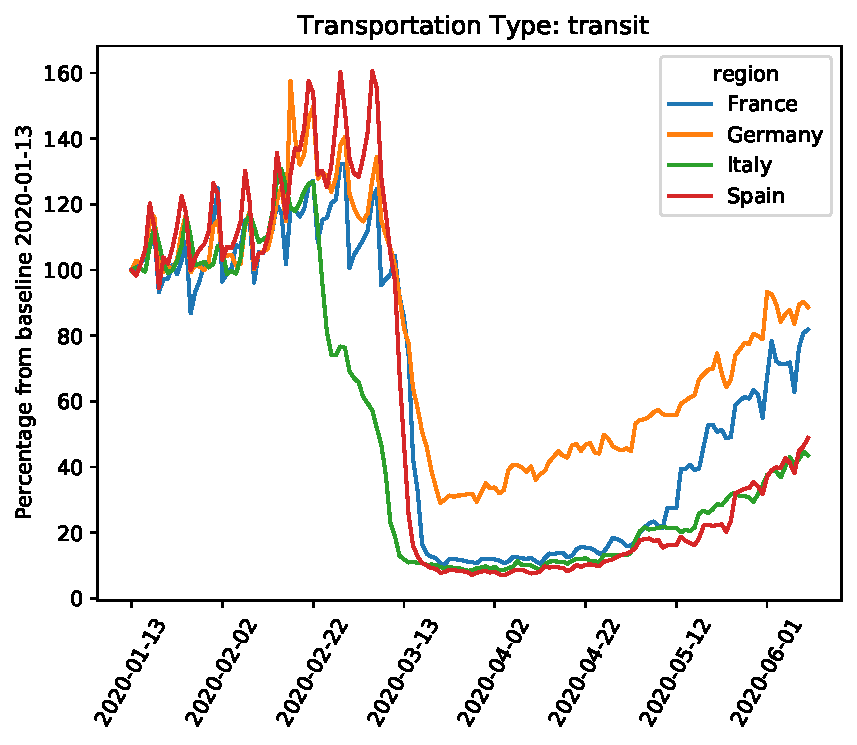
\includegraphics[width=0.5\textwidth]{mobility/apple_demo.pdf}
\caption{Exemplary plot for Apple mobility trend data.}
\label{apple_demo}
\end{figure}

The pre-processing of the Google mobility reports basically follows the same steps. Also the method for handling missing values is the same. In contrast to the Apple datasets, other information types have to be specified here as discussed in the listing above. A demo plot for the movement patterns at workplaces in different European countries is shown in Figure \ref{google_demo}.

\begin{figure}[h]
\centering
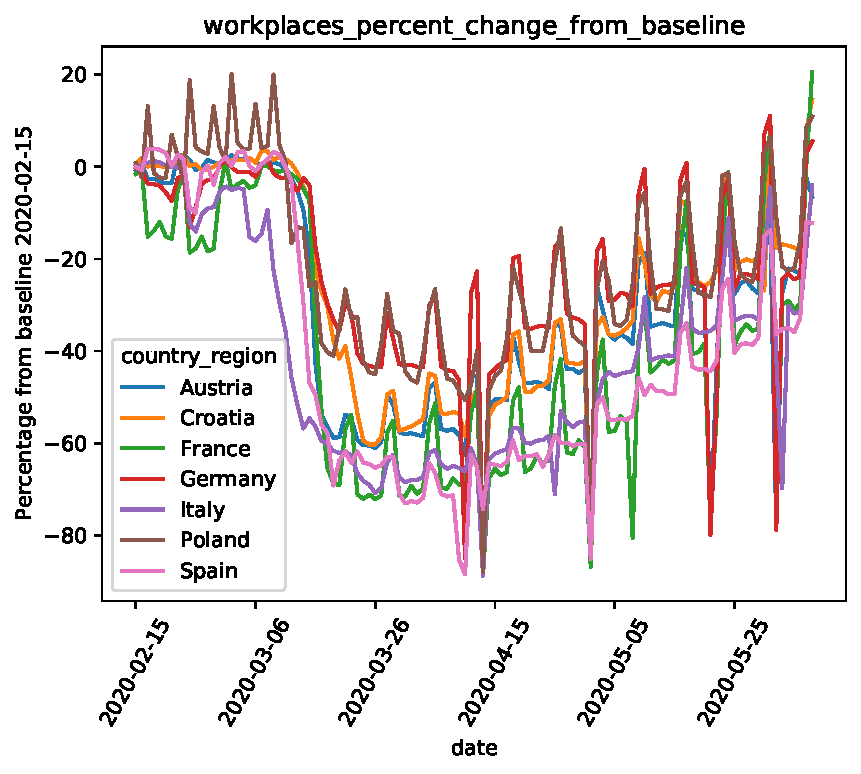
\includegraphics[width=0.5\textwidth]{mobility/google_demo.pdf}
\caption{Exemplary plot for Google mobility report data.}
\label{google_demo}
\end{figure}

Regarding the OpenSky dataset, the pre-processing was computationally more expensive. Since the data were provided in monthly packages, they had to be merged at first. In order to save computational resources, only necessary parts of the dataset were extracted. Since we wanted to extract the overall flight ours per day, the first seen and last seen timestamp was used to calculate the duration of every flight listed in the dataset. Afterwards, a pivot table is created which sums up the flight hours for each day and uses the days as indices. Finally, the day timestamp is modified to only show relevant data. \\
Since these steps take a while when running them on a desktop computer, 
the results were stored in a new csv file containing the overall flight hours per day since January 1st, 2020. The result can be seen in Figure \ref{opensky_demo}.

\begin{figure}[h]
\centering
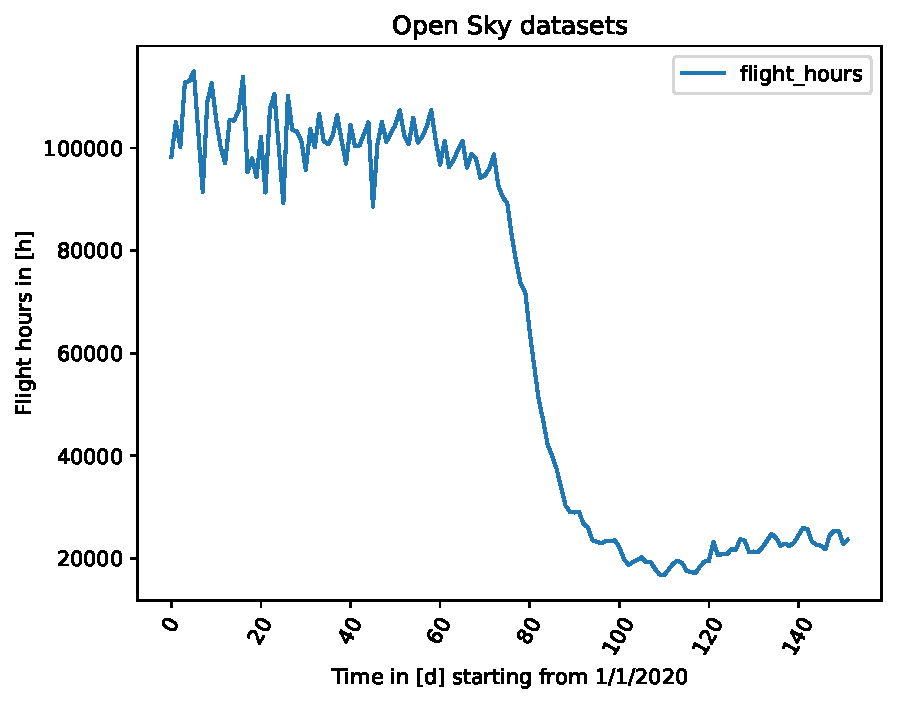
\includegraphics[width=0.5\textwidth]{mobility/opensky_demo.pdf}
\caption{Flight hours per day extracted from the OpenSky datasets.}
\label{opensky_demo}
\end{figure}

The Flightradar24 dataset was already well-prepared. It simply had to be merged into one data frame. The content of this dataset is summarized in Figure \ref{flightradar_demo}. 

\begin{figure}[h]
\centering
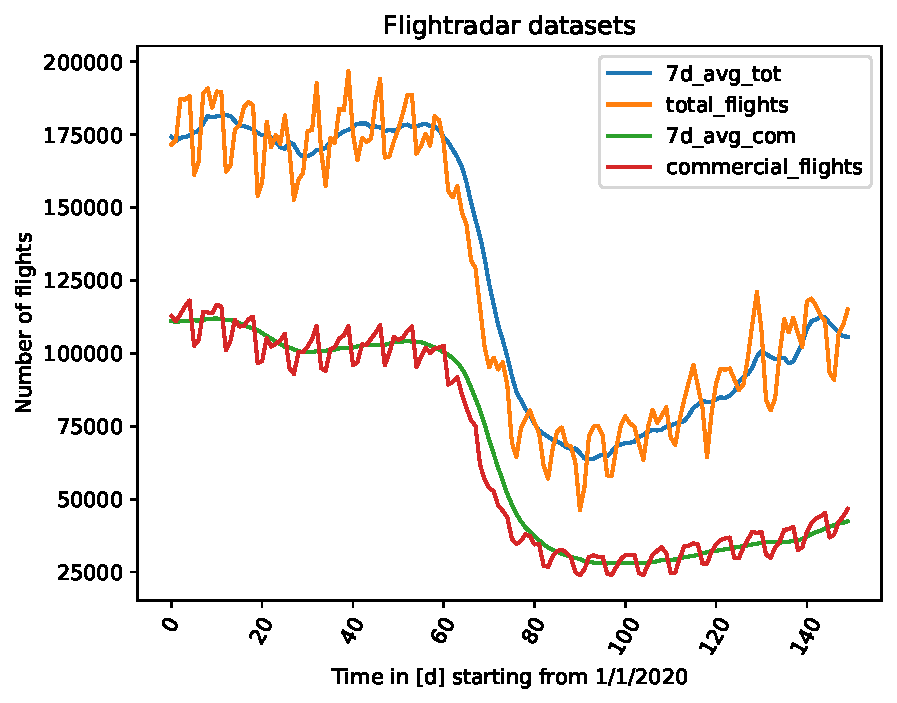
\includegraphics[width=0.5\textwidth]{mobility/flightradar_demo.pdf}
\caption{Number of commercial and total flights provided by Fightradar24.}
\label{flightradar_demo}
\end{figure}

% Check if collected data is useful
All of the collected data might be useful for predicting the influence of COVID-19 on global greenhouse gas emission goals. Especially for predicting the impact in different countries, the mobility report data sets by Apple and Google could be very helpful since they differentiate between movement patterns in different countries. When it comes to transportation, in particular the Apple data set could be very useful because it is separated into different kinds of traveling. This could be extremely useful as different kinds of mobility also have different impacts on greenhouse gas emissions. Together with some side information like the emissions of vehicles, we could try to find correlations between the greenhouse gas levels.

The air traffic data by Flightradar24 has to be reviewed critically. That's because the number of flights does not contain any information about the duration of the flights. Still, it provides an overall intuition about the air traffic and in particular supports the information provided by OpenSky. These datasets could be even more useful since it directly presents how long air planes were flying. Together with the information about average fuel consumption and air plane emissions we can probably use this data to predict the impact of COVID-19 on international climate goals. On the other hand, it has to be taken into consideration that direct emissions from aviation only contribute to about two percent of global emissions \cite{EC_emissions}.

Depending on the machine learning models we are going to use, there will still be some more pre-processing steps required to finally use the datasets for training. One possible strategy to combine the obtained datasets could be to directly take into account the impact of the various contributors to greenhouse gas emissions in percent. This way the information could be combined to one data set. Since we obtained data for various greenhouse gases, this step could also be done for specific greenhouse gases independently in order to improve the accuracy of our predictions. All of the described datasets provide information for roughly the same time interval. The smallest amount of time is covered by the Google data set. That's why an approach for combining the datasets could be to start in February 2020. As it can be seen by inspecting the other datasets which provide information since January 2020, until February the changes in mobility were almost negligible. That's why it will be enough to consider data since February 2020.

% Provide an assessment if you expect the data to be relevant for your project. In what way?
% -> already answered above
